\documentclass[20pt, a0paper, portrait, margin=0mm, innermargin=15mm, blockverticalspace=15mm, colspace=15mm, subcolspace=8mm]{tikzposter}

\usepackage{amsmath, amsthm, amssymb, units, dsfont}
\usepackage{sidecap}
\usepackage{enumerate}
\usepackage{xcolor}

\usepackage{mathtools, mathdots}
\usepackage{pgffor}
\usepackage{pdflscape}
\usepackage{afterpage}
\usepackage{chngcntr}
\usepackage{multirow}
\usepackage{tabulary}

\usepackage{listings}
\usepackage{color}

\usepackage{algorithm}
\usepackage{algorithmic}

\usepackage{breqn}
\usepackage{hyperref}

\usepackage{pgfkeys}

\usepackage{changepage}

\definecolor{darkgreen}{rgb}{0,0.6,0}
\definecolor{darkred}{rgb}{0.6,0,0}
\definecolor{darkblue}{rgb}{0,0,0.6}
\definecolor{darkgrey}{rgb}{0.3,0.3,0.3}
\definecolor{grey}{rgb}{0.6,0.6,0.6} %comment
\definecolor{lightgrey}{rgb}{0.92,0.92,0.92}
\definecolor{terminal}{rgb}{0.9,0.9,0.6}
\definecolor{cmd}{rgb}{0.8,0.8,0.98}
\lstset{ 
        basicstyle=\ttfamily,
%         language=Matlab,                                % choose the language of the code
%       basicstyle=10pt,                                % the size of the fonts that are used for the code
%         numbers=left,                                   % where to put the line-numbers
        keywordstyle=\color{darkblue},
        commentstyle=\color{darkgreen},
        stringstyle=\color{darkred},
%         numberstyle=\footnotesize,                      % the size of the fonts that are used for the line-numbers
        stepnumber=1,                                           % the step between two line-numbers. If it's 1 each line will be numbered
        numbersep=5pt,                                  % how far the line-numbers are from the code
%       backgroundcolor=\color{white},          % choose the background color. You must add \usepackage{color}
        showspaces=false,                               % show spaces adding particular underscores
        showstringspaces=false,                         % underline spaces within strings
        showtabs=false,                                         % show tabs within strings adding particular underscores
%       frame=single,                                           % adds a frame around the code
%       tabsize=2,                                              % sets default tabsize to 2 spaces
%       captionpos=b,                                           % sets the caption-position to bottom
        breaklines=true,                                        % sets automatic line breaking
        breakatwhitespace=false,                        % sets if automatic breaks should only happen at whitespace
        escapeinside={\%*}{*)},                          % if you want to add a comment within your code
        emph={%  
    False, True%
    },emphstyle={\color{darkblue}}
}




%\newcommand{\komentar}[1]{\textcolor{red}{\MakeUppercase{#1}} \newline}
%\newenvironment{upravit}{\color{blue}}{}

\newcommand{\Zomega}{\mathbb{Z}[\omega]}
\newcommand{\Zbeta}{\mathbb{Z}[\beta]}

\newcommand{\ZZ}{\mathbb{Z}}
\newcommand{\QQ}{\mathbb{Q}}
\newcommand{\CC}{\mathbb{C}}
\newcommand{\NN}{\mathbb{N}}
\newcommand{\RR}{\mathbb{R}}


\newcommand{\A}{\mathcal{A}}
\newcommand{\B}{\mathcal{B}}
\newcommand{\Q}{\mathcal{Q}}

\newcommand{\Qw}[3][w]{\Q_{[#1_{-#2}, \dots, #1_{-#3}]}}
\newcommand{\Qwo}[2][w]{\Q_{[#1_{0}, \dots, #1_{-#2}]}}

\newcommand{\tuple}[3][w]{(#1_{-#2}, \dots, #1_{-#3})}
\newcommand{\tupleo}[2][w]{(#1_{0}, \dots, #1_{-#2})}

%\newcommand{\Qb}[1]{\mathcal{Q}_{[b^{#1}]}}
\newcommand{\Qb}[1]{\mathcal{Q}_{[\scriptstyle b]}^{\scriptstyle #1}}

\newcommand{\fin}[1]{\text{Fin}_{#1}(\beta)}

\newcommand{\multMat}[1]{\sum_{i=0}^{d-1} {#1}_i S^i}



\newcommand{\vect}[1]{\begin{pmatrix}
             {#1}_0 \\
             {#1}_1 \\
             \vdots \\
             {#1}_{d-1} 
             \end{pmatrix}}
             
\newcommand{\enum}[1]{({#1}_0,\ldots,{#1}_{d-1})}             

\newcommand{\vertiii}[1]{{\left\vert\kern-0.25ex\left\vert\kern-0.25ex\left\vert #1\right\vert\kern-0.25ex\right\vert\kern-0.25ex\right\vert}}
    
\newcommand{\norm}[2]{\left\lVert#1\right\rVert_{#2}}
\newcommand{\Mnorm}[2]{\vertiii{#1}_{#2}}
\newcommand{\normBeta}[1]{\norm{#1}{\beta}}
\newcommand{\MnormBeta}[1]{\Mnorm{#1}{\beta}}

\renewcommand\Re{\operatorname{Re}}
\renewcommand\Im{\operatorname{Im}}


\renewcommand{\algorithmicrequire}{\textbf{Input:}}
\renewcommand{\algorithmicensure}{\textbf{Ouput:}}
\algsetup{indent=2em}

 \usepackage{pifont}
 \renewcommand\checkmark{\ding{51}}
 \newcommand\xmark{\ding{55}}

 \newcommand{\var}[1]{\textit{#1}}
 \newcommand{\fun}[2]{\textbf{#1}\allowbreak{}(\var{#2})}

 \def\changemargin#1#2{\list{}{\rightmargin#2\leftmargin#1}\item[]}
 \let\endchangemargin=\endlist 


 \newenvironment{method}[2]{
 \noindent \textbf{#1(}\textit{#2}\textbf{)}
 \vspace{-5pt}
 \begin{changemargin}{3em}{0em}}
 {\end{changemargin}}

\def\Cpp{{C\nolinebreak[4]\hspace{-.05em}\raisebox{.4ex}{\tiny\bf ++}}}


 \pgfkeys{
  /phaseOnecaptions array/.is family, /phaseOnecaptions array,
  .unknown/.style = {\pgfkeyscurrentname/.initial = #1},
 }
 
 \newcommand\figurehascaptionOne[1]{\pgfkeys{/phaseOnecaptions array, #1}}
 \newcommand\getcaptionOne[1]{\pgfkeysvalueof{/phaseOnecaptions array/#1}}
 
 \pgfkeys{
  /phase2captions array/.is family, /phase2captions array,
  .unknown/.style = {\pgfkeyscurrentname/.initial = #1},
 }
 
 \newcommand\figurehascaptionTwo[1]{\pgfkeys{/phase2captions array, #1}}
 \newcommand\getcaptionTwo[1]{\pgfkeysvalueof{/phase2captions array/#1}}


% \hyphenation{coef-fi-cient}
% \hyphenation{Algorithm-For-Parallel-Addition}
% \hyphenation{Polynomial-Quotient-Ring}

\hyphenation{con-ver-gen-ce}
\hyphenation{non-con-ver-gen-ce}





\title{Construction of algorithms for parallel addition} 
\author{Jan Legersk\'y} 
\institute{Czech Technical University in Prague}
\usetheme{Autumn}
%\usecolorstyle[colorPalette=BrownBlueOrange]{Germany}

\renewcommand{\Qw}[3][w]{\Q_{[#1_{j-#2}, \dots, #1_{j-#3}]}}
\renewcommand{\Qwo}[2][w]{\Q_{[#1_{j}, \dots, #1_{j-#2}]}}

\renewcommand{\tuple}[3][w]{(#1_{j-#2}, \dots, #1_{j-#3})}
\renewcommand{\tupleo}[2][w]{(#1_{j}, \dots, #1_{j-#2})}


\begin{document}
\maketitle
\begin{columns} 
\column{0.4}
\block{Numeration system}{
	\begin{itemize}
		\item Let $\omega$ be an algebraic integer and let $\Zomega$ be the smallest ring containing $\ZZ$ and $\omega$
		\item Let $\beta\in\Zomega$ be such that $|\beta|>1$ and let $\A\subset\Zomega$ be a finite set containing 0 and 1.
		\item A pair $(\beta, \A)$ is called a \emph{positional numeration system} with \emph{base} $\beta$ and \emph{digit set (alphabet)} $\A$.
		\item A complex number $x$ has a finite \emph{$(\beta, \A)$-representation} if~ there exist digits $x_n,x_{n-1}, \dots x_{-m}\in\A$ such that $x=\sum_{j=-m}^n x_j \beta^j$:
		$$
		(x)_{\beta,\A}= x_n x_{n-1}\cdots x_1 x_0 \bullet x_{-1} x_{-2} \cdots x_{-m}.
		$$
	\end{itemize}
	} 
\block{Addition}{
	$(\beta,\A)$-representations of $x$ and $y$ are summed up digitwise:
	\begin{center}
	\begin{tabular}{ccccclcl}
	$x_{n'}$ & $x_{{n'}-1}$ & $\cdots$ & $x_1$ &$x_0$ &$\bullet$ & $=$& $(x)_{\beta,\A}$ \\%&$x_{-1}$ & $x_{-2}$ & $\cdots$ & $x_{-m'}$ \\
	$y_{n'}$ & $y_{{n'}-1}$ & $\cdots$ & $y_1$ &$y_0$ &$\bullet$ & $=$& $(y)_{\beta,\A}$ \\ \hline % &$y_{-1}$ & $y_{-2}$ & $\cdots$ & $y_{-m'}$ \\ \hline
	$w_{n'}$ & $w_{{n'}-1}$ & $\cdots$ & $w_1$ &$w_0$ &$\bullet$ & $=$& $(x+y)_{\beta,\A+\A}$\,, % &$w_{-1}$ & $w_{-2}$ & $\cdots$ & $w_{-m'}$ \,,
	\end{tabular}	
	\end{center}
	  where
	  $$
	    w_j=x_j+y_j \in \A +\A\,.
	  $$
	  The $(\beta,\A+\A)$-representation $w_{n'} w_{{n'}-1} \cdots w_1 w_0 \bullet$  is converted into $$z_{n} z_{n-1}\cdots z_1 z_0 \bullet=(x+y)_{\beta,\A}\,.$$
	}
	
\block{Digit set conversion from $\A+\A$ into $\A$}{
	A rewriting rule $R(x)= x-\beta$ is used, since $0=q_j \beta^j \cdot R(\beta) =q_j\cdot \beta^{j+1} -\beta  q_j \cdot \beta^{j}$:
	\begin{center}
	\begin{tabular}{rcccccccclcl}
	$w_{n'}$ & $w_{{n'}-1}$ & $\cdots$ & $w_{j+1}$ &\textcolor{red}{$w_{j}$} &$w_{j-1}$ & $\cdots$ & $w_1$ &$w_0$ &$\bullet$ & $=$&$(x+y)_{\beta,\A+\A}$\\
	  &   & &   &  &$q_{j-2}$ & $\iddots$ &  &  &\\
	   &   & &   & \textcolor{red}{$q_{j-1}$}  & $-\beta q_{j-1}$ &  &  &  &\\
	  &   &  $\iddots$&  $q_{j}$ &  \textcolor{red}{$-\beta q_{j}$} & & &  &  &\\ \hline
	$z_{n} \cdots z_{n'}$ & $z_{{n'}-1}$ & $\cdots$ & $z_{j+1}$ &\textcolor{red}{$z_{j}$} &$z_{j-1}$ & $\cdots$ & $z_1$ &$z_0$ &$\bullet$  & $=$&$(x+y)_{\beta,\A}$\\
	\end{tabular}	
	\end{center}
	\coloredbox{The crucial point of any conversion is the choice of the weight coefficient $q_j$ such that $$\textcolor{red}{z_j=w_j + q_{j-1} - q_j \beta} \in \A\,.$$}
	}


\block{Standard vs. parallel conversion}{
	Standard conversion -- \textcolor{red}{$z_j=z_j(w_j, w_{j-1}, \dots, w_0)$}:
   	\begin{center}
	\begin{tabular}{rcccccccccl}
	&$w_{n'}$ & $w_{{n'}-1}$ & $\cdots$ &$w_{j+1}$ &\textcolor{red}{$w_{j}$} &\textcolor{red}{$w_{j-1}$}& \textcolor{red}{$\cdots$}  & \textcolor{red}{$w_1$} &\textcolor{red}{$w_0$} &$\bullet$ \\
	$\longrightarrow z_{n'+1}$ & $z_{{n'}}$ & $z_{n'+1}$&$\cdots$ & $z_{j+1}$ &\textcolor{red}{$z_{j}$} &$z_{j-1}$ & $\cdots$ & $z_1$ &$z_0$ &$\bullet$ \\
	\end{tabular}	
	\end{center}

%   Parallel conversion -- \textcolor{red}{$z_j=z_j(w_{j+t}, \dots, w_{j-r})$} for fixed $r,t\in\NN$ (Avizienis, 1961):
%      	\begin{center}
%	\begin{tabular}{rcccccccccl}
%	$\cdots$&$w_{j+t+1}$ & \textcolor{red}{$w_{j+t}$} & \textcolor{red}{$\cdots$} &\textcolor{red}{$w_{j+1}$} &\textcolor{red}{$w_{j}$} &\textcolor{red}{$w_{j-1}$}& \textcolor{red}{$\cdots$}  & \textcolor{red}{$w_{j-r}$} &$w_{j-r-1}$ &$\cdots$ \\
%	$\longrightarrow \cdots$ & $z_{j+t+1}$ & $z_{j+t}$&$\cdots$ & $z_{j+1}$ &\textcolor{red}{$z_{j}$} &$z_{j-1}$ & $\cdots$ & $z_{j-r}$ &$z_{j-r-1}$ &$\cdots$ \\
%	\end{tabular}	
%	\end{center}
	    
   Parallel conversion with the rewriting rule $x-\beta$ -- \textcolor{red}{$z_j=z_j(w_{j}, \dots, w_{j-r})$} for fixed $r\in\NN$:
      	\begin{center}
	\begin{tabular}{rcccccccccl}
	$\cdots$ &$w_{j+1}$ &\textcolor{red}{$w_{j}$} &\textcolor{red}{$w_{j-1}$}& \textcolor{red}{$\cdots$}  & \textcolor{red}{$w_{j-r}$} &$w_{j-r-1}$ &$\cdots$ \\
	$\longrightarrow \cdots$  & $z_{j+1}$ &\textcolor{red}{$z_{j}$} &$z_{j-1}$ & $\cdots$ & $z_{j-r}$ &$z_{j-r-1}$ &$\cdots$ \\
	\end{tabular}	
	\end{center}
	}


\column{0.6}



\block{Extending window method}{
	The length of window $r$ and a weight function $q:(\A+\A)^{r} \rightarrow \Q \subset \Zomega$ such that $q_j=q(w_j, \dots, w_{j-(r-1)})$ are determined in two phases:
    \begin{enumerate}
        \item The weight coefficients set $\Q$ is constructed as a finite subset of $\Zomega$.
        \item The length of window $r$ is extended and a weight coefficient from $\Q$ is tried to be found for all $(w_j,w_{j-1}, \dots , w_{j-(r-1)}) \in (\A+\A)^{r}$ to define the weight function $q$.
    \end{enumerate}
}

\begin{subcolumns}
\subcolumn{0.35}
\block{Phase 1}{
We construct the set $\Q$ such that
            $$
    		\underbrace{(\A+\A)}_{w_j \in}+ \underbrace{\Q}_{q_{j-1} \in} \subset \underbrace{\A}_{z_j \in} + \underbrace{\beta \Q}_{\beta q_j \in}
    		$$
  \begin{algorithmic}[0]
    \STATE $k:=0$ 
    \STATE $Q_0:=\{0\}$
    \REPEAT
     \STATE  Extend $\Q_k$ to $\Q_{k+1}$ so that $$\A+\A+ \Q_k \subset \A + \beta \Q_{k+1}$$
     \vspace{-30pt}
      \STATE  $k:=k+1$
      \UNTIL{$\Q_k = \Q_{k+1}$}      
      \STATE $\Q:=\Q_k$
  \end{algorithmic}
}
\subcolumn{0.65}
\block{Phase 2}{
  \begin{algorithmic}[0]
    \FORALL{$w_j \in \A+\A$}
            \STATE Find set $\Q_{[w_{j}]} \subset \Q$ such that
              $$
              w_j + \Q \subset \A + \beta \Q_{[w_{j}]}\,.
              $$\vspace{-20pt}
    \ENDFOR
    \STATE $k:=0$
    \WHILE{$\max\{\#\Qwo{k}:\tupleo{k} \in(\A+\A)^{k+1} \} > 1$}
        \STATE $k:= k +1$
        \FORALL{$\tupleo{k} \in (\A+\A)^{k+1}$}
            \STATE Find set $\Qwo{k} \subset \Qwo{(k-1)}$ such that
              $$
              w_j + \Qw{1}{k} \subset \A + \beta \Qwo{k}\,.
              $$\vspace{-20pt}
        \ENDFOR  
    \ENDWHILE  
    \STATE $r:= k$ 
    \FORALL{$\tupleo{(r-1)}\in(\A+\A)^{r}$}
	    \STATE $q\tupleo{(r-1)}:=$ only element of $\Qwo{r}$
	\ENDFOR
  \end{algorithmic}
}
\end{subcolumns}

\block{Alphabet}{
	Let $\A\subset\Zbeta$. If the extending window method with the rewriting rule $x-\beta$ converges for the numeration system $(\beta, \A)$, then 
	$$
	\#\A \geq \max \{|m_\beta(0)|, |m_\beta(1)|\}\,.
	$$
	Moreover, if $\beta$ is such that it has a real conjugate greater than 1, then 
	$$
	\#\A \geq \max \{|m_\beta(0)|, |m_\beta(1)|+2\}\,.
	$$
}


\block{Convergence of Phase 1}{
	If the extending window method with the rewriting rule $x-\beta$ converges for the numeration system $(\beta, \A)$, then the base $\beta$ is expanding.

\vspace{20pt}

	Let $\A$ contain at least one representative of each congruence class modulo $\beta$ in $\Zomega$. If $\beta$ is expanding, then Phase 1 of the extending window method converges.
}



\block{Convergence of Phase 2}{
If number of possible weight coefficients for input digits $bbb\dots$ does not decrease for some $b\in\A+\A$ when the length of window is increased, then Phase 2 does not converge.

\vspace{20pt}
If there is an infinite path in the graph which is defined by non-decreasing combinations, then Phase 2 does not converge.
}
\end{columns}

\block{Eisenstein base $\beta = -\frac{3}{2} + \frac{\imath \sqrt{3}}{2}$ with the complex alphabet $\A =\{0, 1, -1, \omega, -\omega, -\omega - 1, \omega + 1\}$}{
\begin{tikzfigure}
    \centering
    %\caption{Construction of the weight coefficients set $\Q$, input alphabet $\B=\A+\A$}
    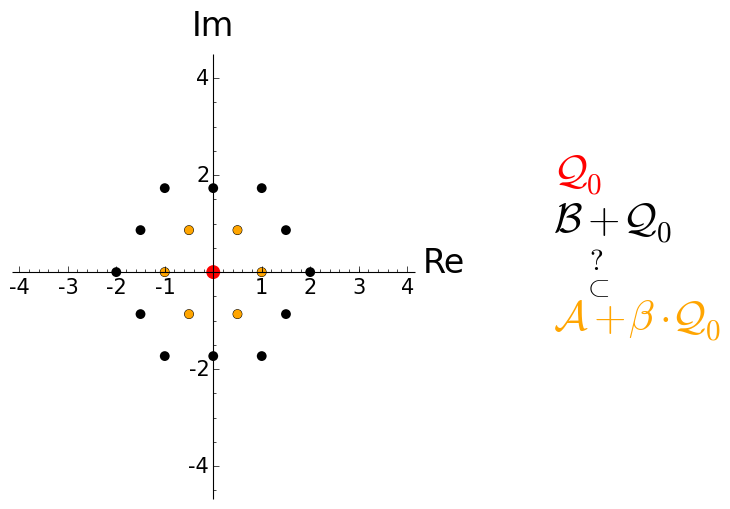
\includegraphics[width=0.18\textwidth]{img/eisenstein/phase1_image_3.png}
    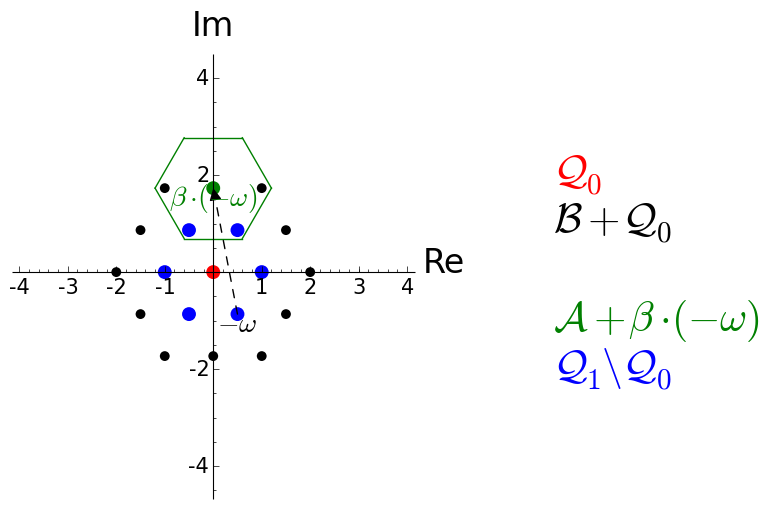
\includegraphics[width=0.18\textwidth]{img/eisenstein/phase1_image_4.png}
    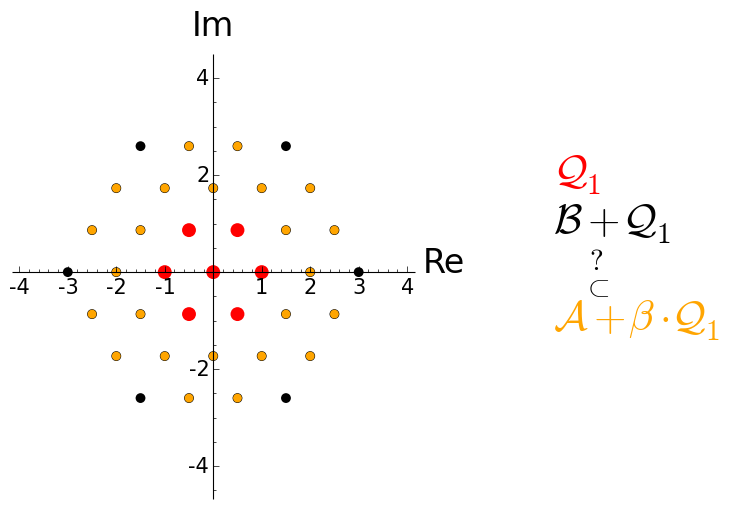
\includegraphics[width=0.18\textwidth]{img/eisenstein/phase1_image_6.png}
    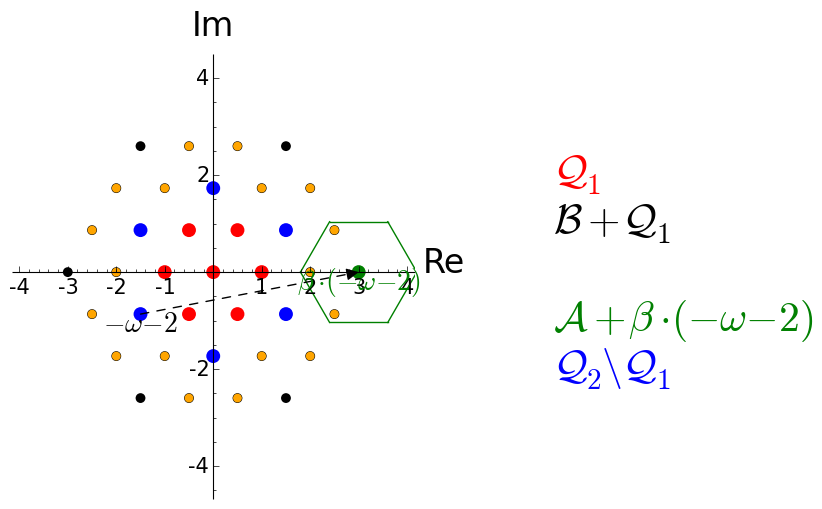
\includegraphics[width=0.18\textwidth]{img/eisenstein/phase1_image_7.png}
    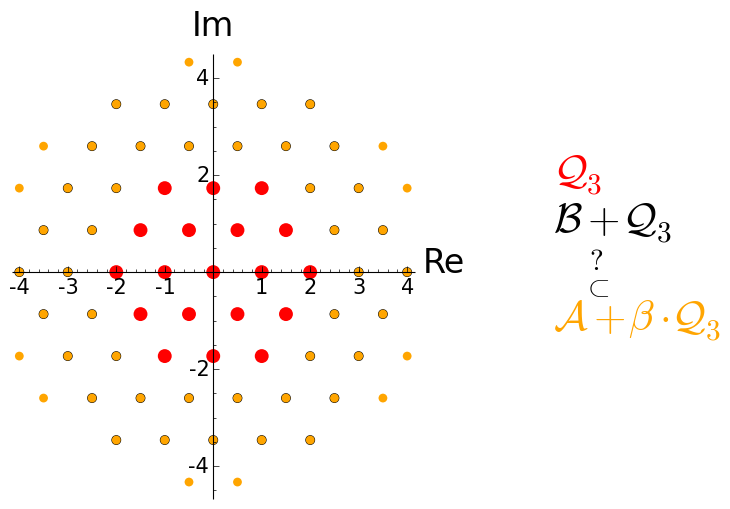
\includegraphics[width=0.18\textwidth]{img/eisenstein/phase1_image_12.png}
\end{tikzfigure}


%The construction of set $\Q_{[\omega,1,2]}$ for the Eisenstein base $\beta = -\frac{3}{2} + \frac{\imath \sqrt{3}}{2}$ with the complex alphabet $\mathcal{A} =\{0, 1, -1, \omega, -\omega, -\omega - 1, \omega + 1\}$  and input alphabet $\B=\A+\A$ is illustrated on Figures \ref{img:phase2img1} -- \ref{img:phase2img7}. See also Example \ref{ex:Eisenstein1-blockcomplex}.
%\label{app:phase2}    
%
%\figurehascaptionTwo{1 = Phase 2 starts with the weight coefficients set $\Q$ from Phase 1.}
%\figurehascaptionTwo{2 = The set $\omega+\Q$ need to be covered.}
%\figurehascaptionTwo{3 = The elements of $\omega+\Q$ are covered by the set $\Q_{[\omega]}\subset\Q$.}
%\figurehascaptionTwo{4 = The set $\omega+\Q_{[1]}$ need to be covered.}
%\figurehascaptionTwo{5 = The elements of $\omega+\Q_{[1]}$ are covered by the set $\Q_{[\omega,1]}\subset\Q_{[\omega]}$.}
%\figurehascaptionTwo{6 = The set $\omega+\Q_{[1,2]}$ need to be covered.}
%\figurehascaptionTwo{7 = The elements of $\omega+\Q_{[1]}$ are covered by the set $\Q_{[\omega,1,2]}\subset\Q_{[\omega,1]}$ which has only one element{.} This element is the output of the weight function $q{(\omega,1,2)}$.}
%
%
%
%\foreach \n in {1,...,7} {%
%\begin{SCfigure}[][htbp]
%    \centering
%    \caption{\getcaptionTwo{\n}}
%    \label{img:phase2img\n}
%    \includegraphics[height=0.3\textheight]{img/eisenstein/phase2_image_\n.png}
%\end{SCfigure}
%    }
%    
}

\block{Testing}{
    \begin{tabular}{l|c cc| c c c} 
 $\omega$                & Base                                                    & $\#\A$ & $m_\beta$ & Phase 1 & bbb & Phase 2 \\ \hline
$1/2\cdot I\sqrt{15} - 1/2 $ & $  \omega $ & $  6    $ & $  x^2 + x + 4     $  & \checkmark      & \checkmark  & \xmark  \\ \hline
$1/2\cdot I\sqrt{11} + 1/2 $ & $  -2\omega - 2  $ & $  27   $ & $  x^2 + 6x + 20    $  & \checkmark      & \checkmark  & \checkmark      \\
$1/2\cdot I\sqrt{11} + 1/2 $ & $  -\omega+ 1  $ & $  3    $ & $  x^2 - x + 3  $  & \checkmark      & \checkmark  & \xmark  \\ \hline
$1/2\cdot I\sqrt{7} - 1/2  $ & $  \omega  $ & $  4    $ & $  x^2 + x + 2    $  & \checkmark      & \checkmark  & \checkmark      \\
$1/2\cdot I\sqrt{7} + 1/2  $ & $  \omega    $ & $  2    $ & $  x^2 - x + 2      $  & \checkmark      & \checkmark  & \xmark  \\
$1/2\cdot I\sqrt{7} + 3/2  $ & $  \omega                                                   $ & $  4    $ & $  x^2 - 3x + 4                                              $& \checkmark  & \xmark  & -     \\ \hline
%$1/2\cdot I\sqrt{3} - 1/2  $ & $  2\omega                                                 $ & $  8    $ & $  x^2 + 2x + 4                                          $  & \checkmark      & \checkmark  & \checkmark      \\
$I\sqrt{3}            $ & $  -\omega                                                  $ & $  4    $ & $  x^2 + 3                                                $  & \checkmark      & \checkmark  & \checkmark      \\
$1/2\cdot I\sqrt{3} + 1/2  $ & $  -3\omega + 2                                            $ & $  7    $ & $  x^2 - x + 7                                            $  & \checkmark      & \checkmark  & \xmark  \\ \hline
$I\sqrt{2}            $ & $  -\omega                                                  $ & $  3    $ & $  x^2 + 2                                                $  & \checkmark      & \checkmark  & \checkmark      \\
%$I\sqrt{2} + 1        $ & $  -\omega  - 3  $ & $  27   $ & $  x^2 + 8x + 18                                         $  & \checkmark      & \checkmark  & \checkmark      \\
$I\sqrt{2} - 1        $ & $  \omega                                                   $ & $  6    $ & $  x^2 + 2x + 3                                          $  & \checkmark      & \checkmark  & \xmark  \\ \hline
$I - 1                $ & $  \omega                                                   $ & $  5    $ & $  x^2 + 2x + 2                                          $  & \checkmark      & \checkmark  & \checkmark      \\
$I                    $ & $  -3\omega                                                $ & $  10   $ & $  x^2 + 9                                                $  & \checkmark      & \checkmark  & \xmark  \\ \hline
$-1/2\sqrt{5} + 3/2   $ & $  -2\omega - 2                                            $ & $  31   $ & $  x^2 + 10x + 20                                        $  & \checkmark      & \checkmark  & \checkmark      \\
$-1/2\sqrt{5} + 3/2   $ & $  3\omega   - 3 $ & $  13   $ & $  x^2 - 3x - 9                                          $  & \checkmark      & \checkmark  & \xmark  \\ \hline
$1/2\sqrt{13} - 3/2   $ & $  \omega   - 3   $ & $  27   $ & $  x^2 + 9x + 17                                         $  & \checkmark      & \checkmark  & \xmark  \\
$1/2\sqrt{13} + 1/2   $ & $  -2\omega + 2                                            $ & $  16   $ & $  x^2 - 2x - 12                                         $  & \checkmark      & \xmark  & -  \\ \hline
$1/2\sqrt{17} - 3/2   $ & $  \omega   - 3   $ & $  26   $ & $  x^2 + 9x + 16                                         $  & \checkmark      & \checkmark  & \checkmark           
 \end{tabular}
}
\end{document}